\begin{enumerate}
	\item Exercício
	
	$z = f(x, y) = y\e^x;\; dz = dx dy$\newline\newline
	$v = \integral_2^4 \integral_1^9 z\, dz = \integral_2^4 \integral_1^9 y\e^x\, dy dx = \integral_2^4 \e^x\, dx \integral_1^9 y\, dy = \integral_2^4 \e^x\, dx \left[\dfrac{y^2}{2}\right]_1^9 = \integral_2^4 \e^x\, dx \dfrac{1}{2}\left[y^2\right]_1^9 = \dfrac{1}{2}\integral_2^4 \e^x\, dx \left[9^2 - 1^2\right] = 40\integral_2^4 \e^x\, dx = 40\left[\e^x\right]_2^4 = 40\left[\e^4 - \e^2\right] = 40e^2\left(e^2 - 1\right)$\newline
	
	\item Exercício
	
	$z = f(x,y) = x^2y^3;\; dz = dx dy$\newline\newline
	$v = \integral_0^1 \integral_2^4 z\, dz = \integral_0^1 \integral_2^4 x^2y^3\, dx dy = \integral_0^1 x^2\, dx \integral_2^4 y^3\, dy = \integral_0^1 x^2\, dx \left[\dfrac{y^4}{4}\right]_2^4 = \dfrac{1}{4}\integral_0^1 x^2\, dx \left[y^4\right]_2^4 = \dfrac{1}{4}\integral_0^1 x^2\, dx \left[4^4 - 2^4\right] = \dfrac{1}{4}\integral_0^1 x^2\, dx \left[2^8 - 2^4\right] = \dfrac{1}{4}\integral_0^1 x^2\, dx \left[2^4\left(2^4 - 1\right)\right] = \dfrac{1}{4}\integral_0^1 x^2\, dx \left[16 \cdot 15\right] = 60\integral_0^1 x^2\, dx = 60 \left[\dfrac{x^3}{3}\right]_0^1 = 20 \left[x^3\right]_0^1 = 20 \left[1^3 - 0^3\right] = 20 \cdot 1 =  20$\newline
	
	\item Exercício
	
	$\integral \integral_D (x + 2y) da$\newline\newline
	\textrm{D} = Região limitada pela parábola $y = x^2 + 1$ e as retas $x = -1$ e $x = 2$.\newline\newline
	$z = f(x,y) = x + 2y;\; da = dz = dx dy$\newline
	
	\begin{figure}[H]
		\centering
		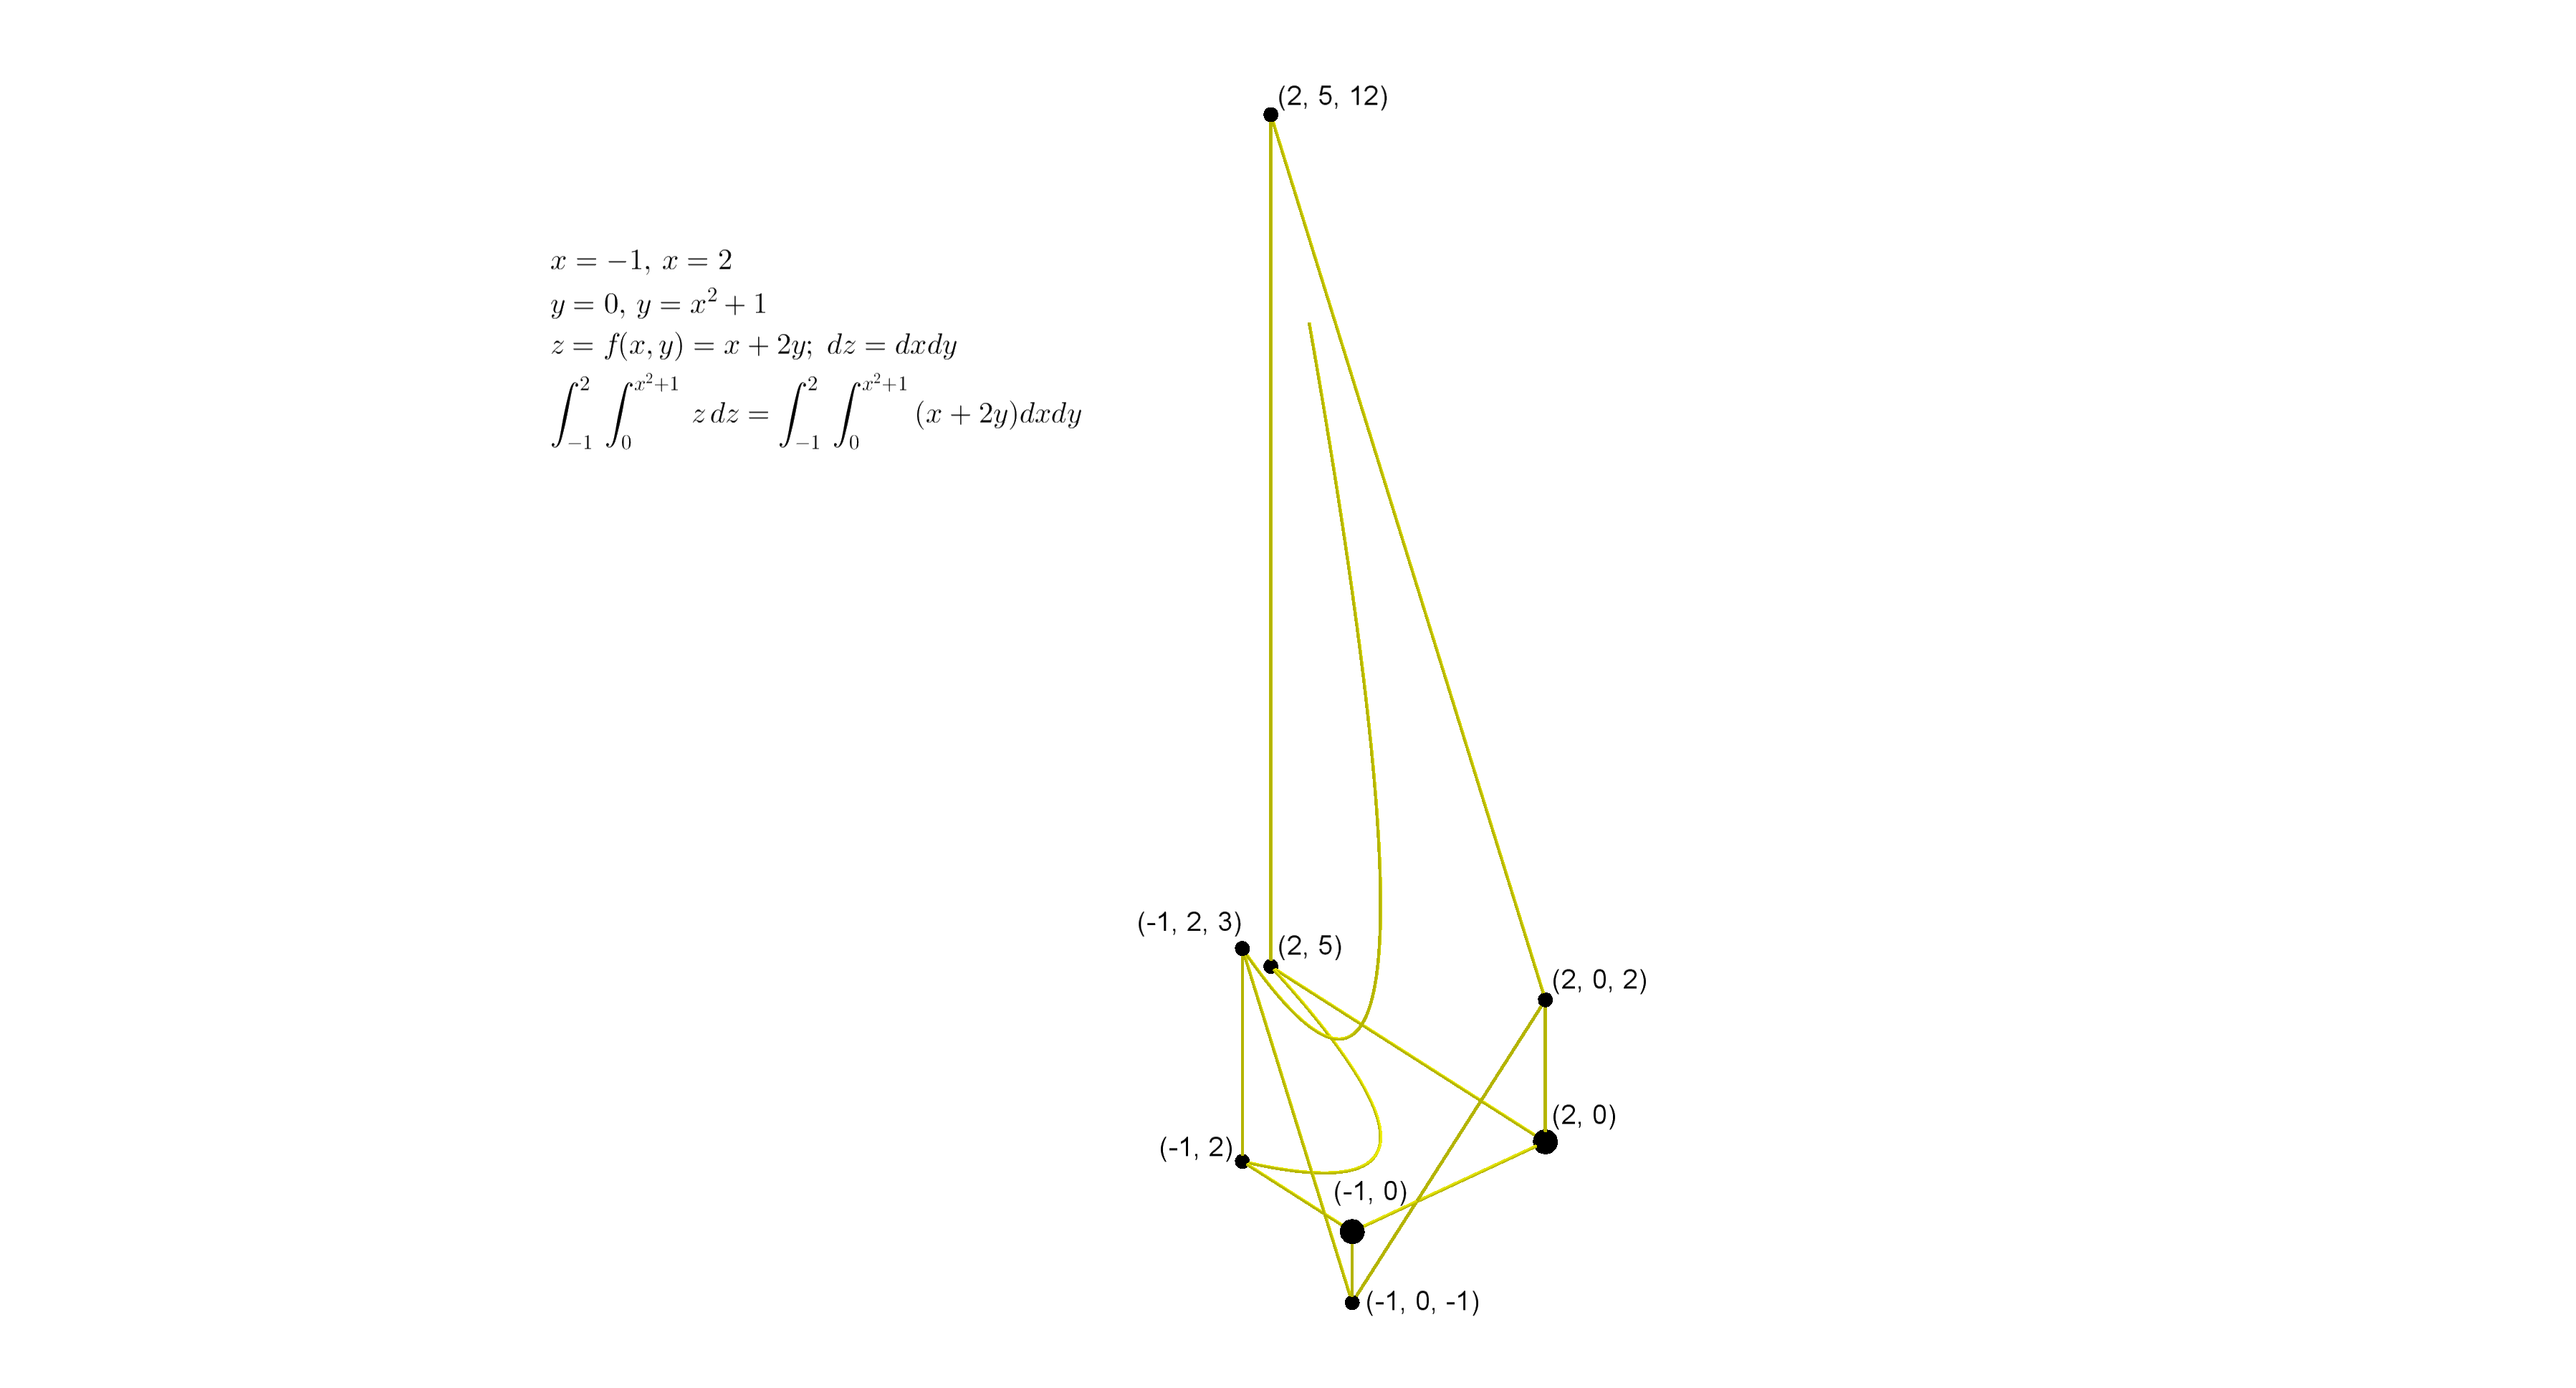
\includegraphics[width=\textwidth]{v01_a04_e03.png}
		\caption{Integrais duplas - Aula 4 - Exercício III}
		\label{v01_a04_e03}
	\end{figure}
	
	$\integral_{-1}^2 \integral_0^{x^2 + 1} z\, dz = \integral_{-1}^2 \integral_0^{x^2 + 1} (x + 2y) dx dy = \integral_{-1}^2 dx \integral_0^{x^2 + 1} (x + 2y) dy = \integral_{-1}^2 dx \left(x\integral_0^{x^2 + 1} dy + 2\integral_0^{x^2 + 1} y\, dy\right) = \integral_{-1}^2 dx \left[xy + \overstrike{2}\dfrac{y^2}{\overstrike{2}}\right]_0^{x^2 + 1} = \integral_{-1}^2 dx \left[y(x + 2y)\right]_0^{x^2 + 1} = \integral_{-1}^2 dx \left[\left(x^2 + 1\right)\left[x + 2\left(x^2 + 1\right)\right] \overstrike{- 0(x + 2\cdot0)}\right] = \integral_{-1}^2 dx \left[\left(x^2 + 1\right)\left(2x^2 + x + 2\right)\right] = \integral_{-1}^2 dx \left(2x^4 + x^3 + 4x^2 + x + 2\right) = 2\integral_{-1}^2 x^4\, dx + \integral_{-1}^2 x^3\, dx + 4\integral_{-1}^2 x^2\, dx + \integral_{-1}^2 x\, dx + 2\integral_{-1}^2 dx = \left[2\dfrac{x^5}{5} + \dfrac{x^4}{4} + 4\dfrac{x^3}{3} + \dfrac{x^2}{2} + 2x\right]_{-1}^2 =\\ \left[\dfrac{24x^5 + 15x^4 + 80x^3 + 30x^2 + 120x}{60}\right]_{-1}^2 = \dfrac{1}{60}\left[x\left(24x^4 + 15x^3 + 80x^2 + 30x + 120\right)\right]_{-1}^2 = \dfrac{1}{60}\left[2\left(24\cdot2^4 + 15\cdot2^3 + 80\cdot2^2 + 30\cdot2 + 120\right) \right.\\\left.- (-1)\left(24(-1)^4 + 15(-1)^3 + 80(-1)^2 + 30(-1) + 120\right)\right] =\\ \dfrac{1}{60} [2(384 + 120 + 320 + 60 + 120) + (24 - 15 + 80 - 30 +120)] = \dfrac{1}{60} (2008 + 179) = \dfrac{2187}{60} = \frac{729}{20} = 36,45$ 
\end{enumerate}